\setlength{\footskip}{8mm}

\chapter{METHODOLOGY}


\section{Architectureal Overview}

Longitudinal medical image comparison requires models to distinguish true pathological evolution from stochastic acquisition variability, such as patient movement or differences in posture. Conventional Difference-aware Medical VQA methods rely on direct feature subtraction, which implicitly assumes perfect spatial correspondence between scans. This thesis introduces ALIGN-VQA, an alignment-guided residual modeling architecture designed to overcome these spatial misalignment vulnerabilities.

\begin{figure}[htbp]
	\centering
	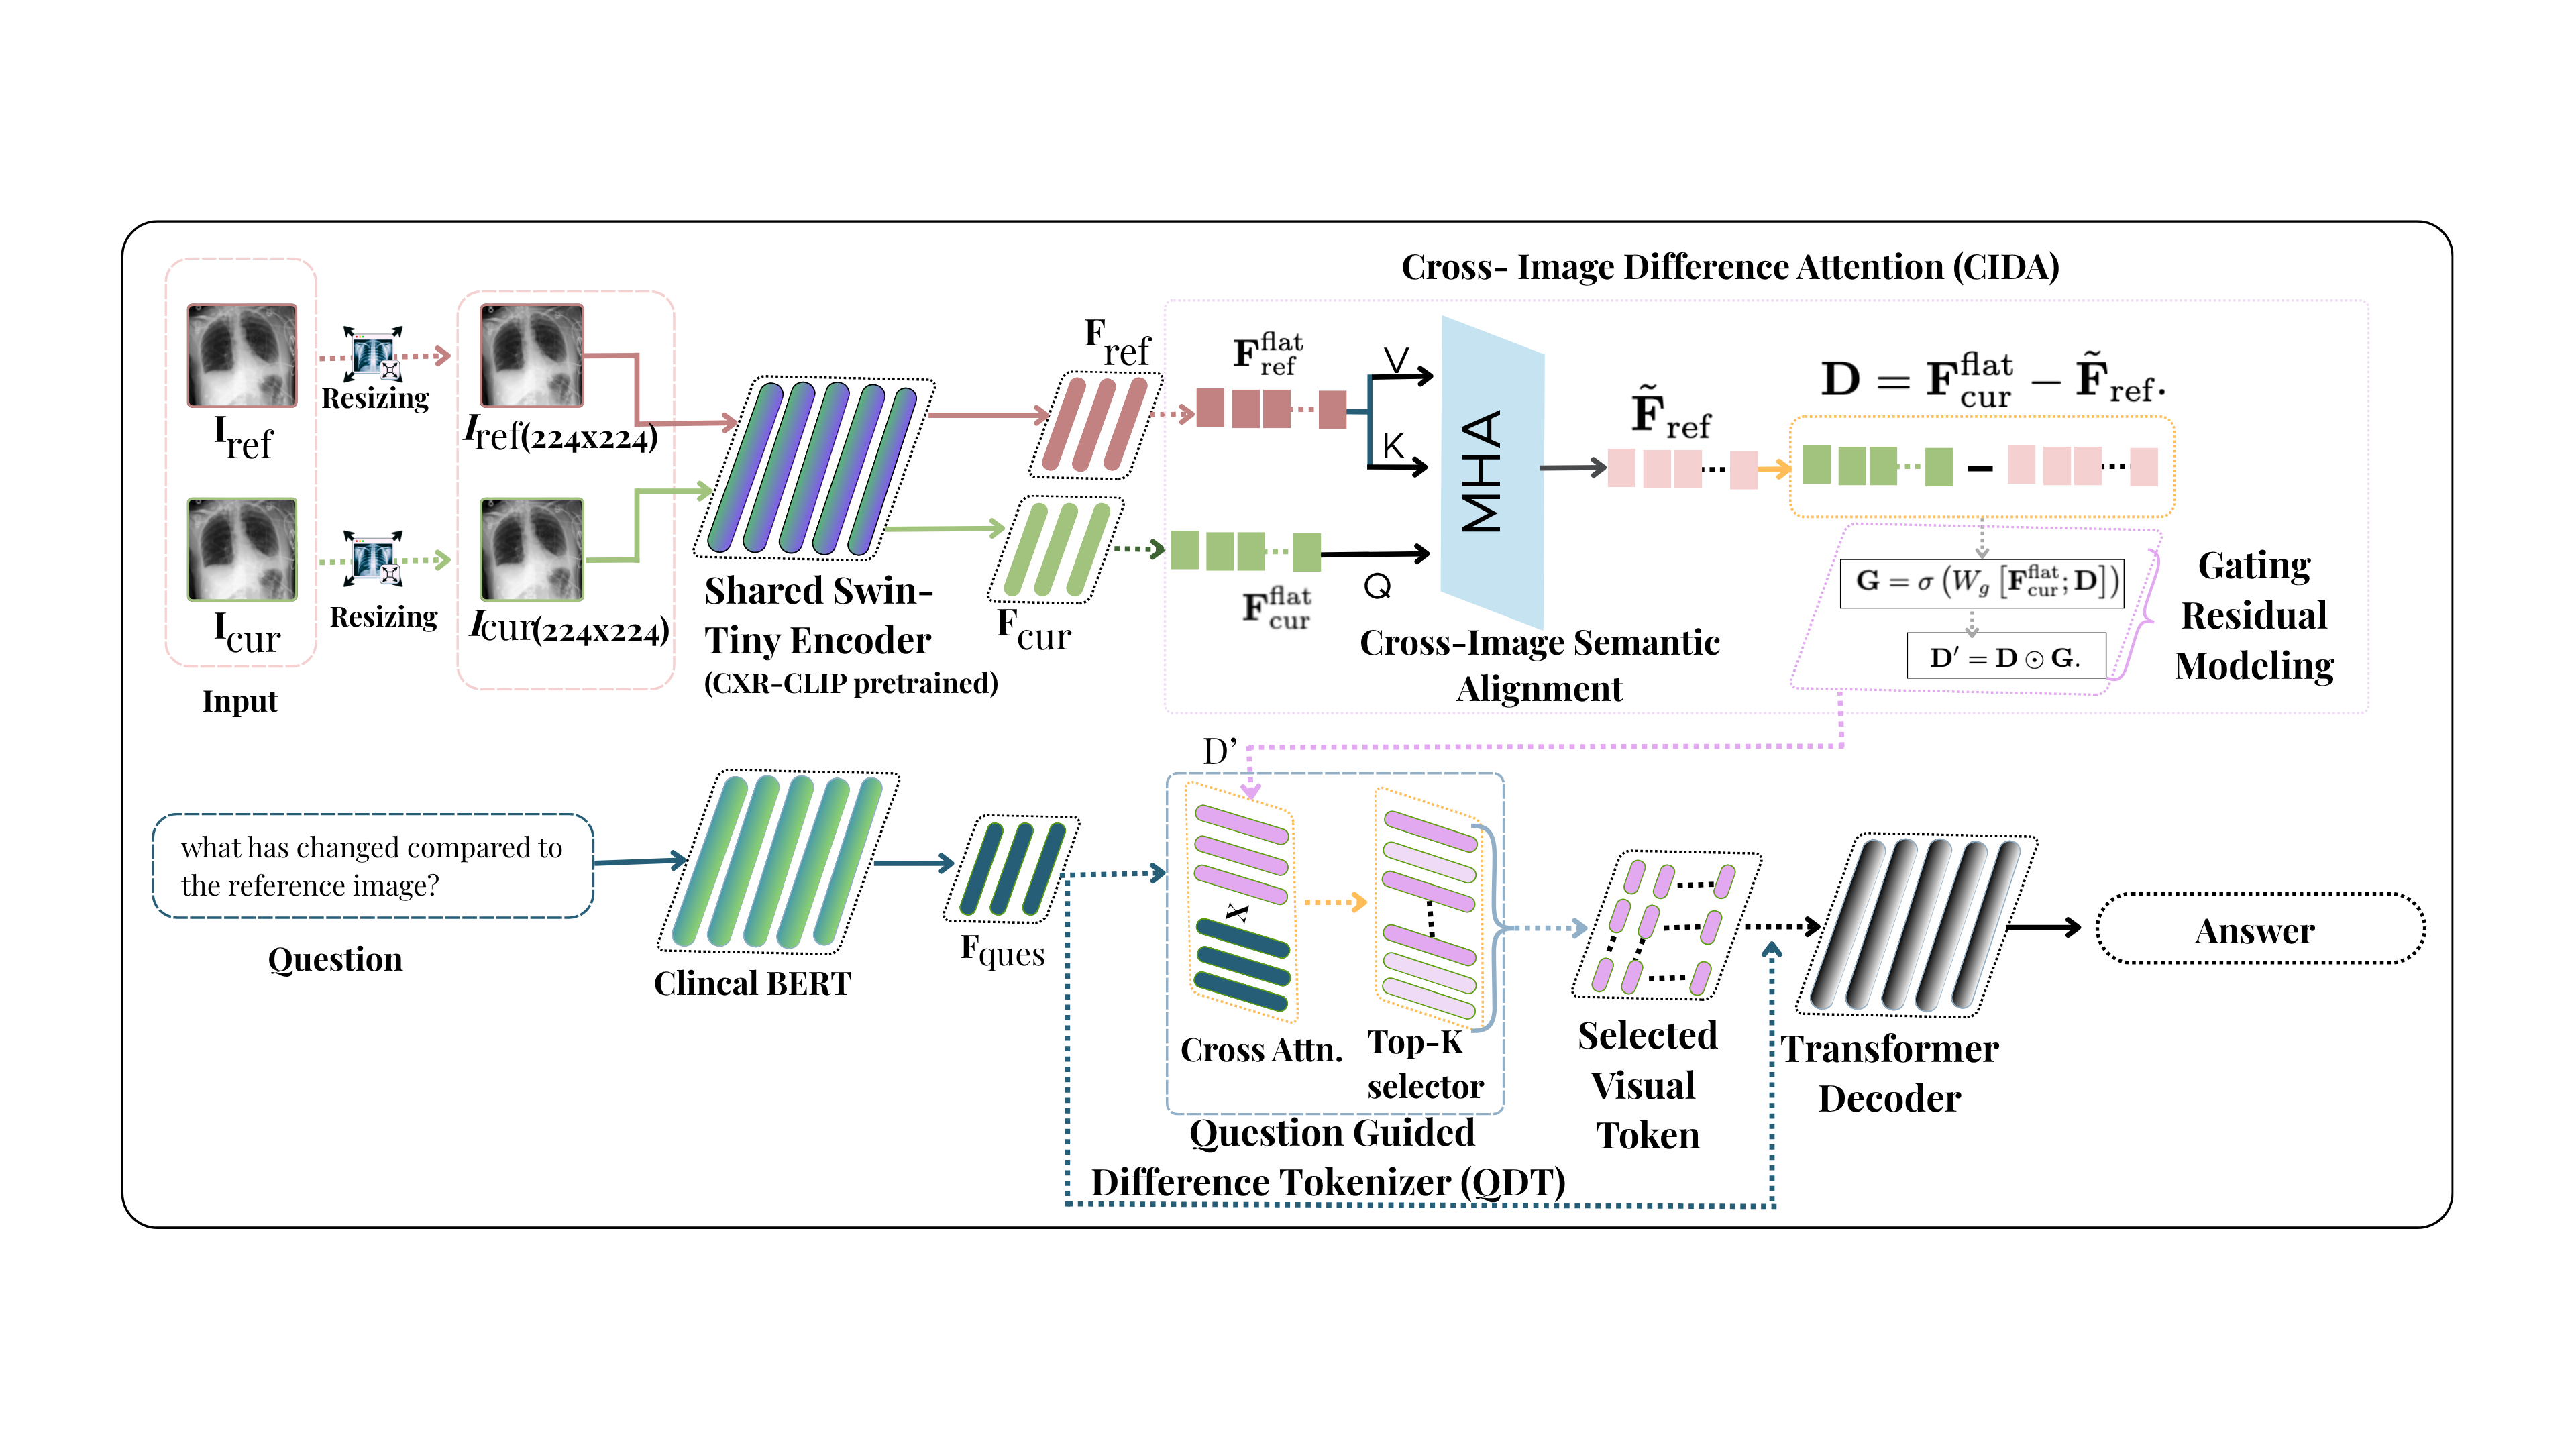
\includegraphics[width=0.9\textwidth]{figures/high_architecture.png}
	\caption{High Level Architecture Overview}
	\label{fig:high_architecture}
\end{figure}

As illustrated in Figure \ref{fig:high_architecture}, the proposed methodology shifts from a brute-force comparison paradigm to an efficient, explicit reasoning framework. The architecture is composed of three primary functional blocks. Cross-Image Difference Attention (CIDA) and gated residual modeling semantically reconstructs and aligns historical features to the current scan before isolating evolution-aware deviations. Question-Guided Difference Tokenizer (QDT) employs cross-attention to selectively pool a sparse, highly relevant set of temporal changes based on the clinical query. Conditional answer generation and multi-stage training utilizes a lightweight transformer decoder optimized through a highly structured multi-stage training strategy to ensure grounded, halucination-free reasoning.

\section{Problem Formulation}
Given a patient's historical reference X-ray $I_{ref}$, a current follow-up X-ray $I_{cur}$, and a clinically grounded question $Q$, the objective of the Diff-VQA system is to generate an accurate natural language answer $\hat{A}$ describing the temporal evolution of the targeted pathology. Instead of mapping inputs directly to a dense difference map, our formulation isolates question-relevant residual deviations to conditionally autoregress the answer.

\section{Architectural Components}

\subsection{Visual Feature Extraction}
The visual processing pipeline begins by encoding the paired longitudinal images. Both $I_{ref}$ and $I_{cur}$ are resized to $224 \times 224$ and passed through a shared tiny variant of \cite{swin}. The shifted-window self-attention mechanism within the encoder enables highly efficient local-to-global context modeling. To inject domain-specific radiographic priors immediately into the feature extraction phase, the backbone is initialized with pretrained weights from \cite{cxr-clip}. This process yields two feature maps, which are flattened into token sequences:
\begin{equation}
	F_{ref}^{flat}, F_{cur}^{flat} \in \mathbb{R}^{B \times N \times C}
\end{equation}
where $B$ is the batch size, $C$ is the channel dimension, and $N = H \times W$ represents the number of spatial patches.

\subsection{Cross Image Difference Attention}
To compensate for spatial misalignments resulting from varying patient positioning and inspiratory effort between visits, we introduce the CIDA module. It utilizes Multi-Head Cross-Attention (MHA) to semantically align the historical features to the coordinate space of the current image. Specifically, the current image features are utilized as queries ($Q$), while the reference image features serve as keys ($K$) and values ($V$):
\begin{equation}
	\tilde{F}_{ref} = \text{MHA}(F_{cur}^{flat}, F_{ref}^{flat}, F_{ref}^{flat})
\end{equation}
This operation reconstructs an aligned historical representation ($\tilde{F}_{ref}$) that is spatially coherent with the current scan, creating a reliable foundation for calculating true temporal differences.

\subsection{Learnable Gated Residual Modeling}
Once the features are aligned, the raw residual deviation is computed via element-wise subtraction:
	\begin{equation}
		D = F_{cur}^{flat} - \tilde{F}_{ref}
	\end{equation}
Because medical imaging inherently contains acquisition noise, utilizing the raw residual $D$ directly can mislead downstream modules. Therefore, a learnable gating mechanism is applied. The gate calculates a channel-wise importance filter by concatenating the current features with the raw residual and passing them through a projection matrix $W_g$ and a sigmoid function $\sigma$:
	\begin{equation}
		G = \sigma(W_g[F_{cur}^{flat} ; D])
	\end{equation}
The refined, evolution-aware residual features are then extracted via element-wise multiplication:
	\begin{equation}
		D' = D \odot G
	\end{equation}
The resulting tokens $\{D'_i\}_{i=1}^N$ encode clean, structured temporal changes.

\subsection{Domain-Aware Text Encoding}
The clinical question $Q$ is encoded using \cite{bio-clinical-bert}, a language model extensively pretrained on clinical notes. This provides a domain-aware question embedding vector $F_{ques} \in \mathbb{R}^C$ that captures the semantic nuance of radiological terminology such as distinguishing between consolidation and atelectasis.

\subsection{Question-Guided Difference Tokenization}
Standard Diff-VQA models process all spatial tokens, which dilutes the signal of localized pathologies. The QDT module solves this by selectively pooling only the temporal changes that are relevant to the specific clinical question.Attention weights ($\alpha_i$) are computed between the question embedding $F_{ques}$ and each visual residual token $D'_i$ using dot-product attention. To enforce extreme token sparsity and computational efficiency, a hard Top-K selection mechanism is applied:
\begin{equation}
	T_{vis} = \text{TopK}(\{\alpha_i D'_i\})
\end{equation}
Based on empirical ablations, $K$ is set to 16, ensuring the model forwards only the most highly discriminative visual evidence to the language decoder.

\subsection{Conditional Answer Generation}
The final response generation relies on a lightweight standard transformer decoder. The selected sparse visual tokens $T_{vis}$ are concatenated with the question embedding $F_{ques}$. The decoder autoregressively predicts the answer $\hat{A}$ step-by-step, conditioned strictly on the question semantics and the isolated, aligned temporal changes.

\subsection{Counterfactual Regularizer}
To mitigate the model's tendency to hallucinate, a counterfactual regularizer (CFA-Reg) is introduced. For each training sample $(I_{cur},I_{ref}, Q, A)$, we generate a logical opposite by either swapping the images $(I_{ref},I_{cur})$ or negating a directional term in the question (e.g., "worsened" → "improved"). The model performs a forward pass on both the real and counterfactual inputs, generating two distinct answer distributions, $P_{real}$ and $P_{cofa}$.


\subsection{Masked Residual Modeling}
The masked residual modeling (MRM) process is designed to force the model to learn the contextual structure of the difference maps. First, an unlabeled image pair $(I_{cur}, I_{ref})$ is passed through the vision encoder to generate the concatenated residual map, $R$. A significant portion of the patches in this map are then randomly masked. The unmasked patches are fed into the QDT's vision backbone, which is tasked with predicting the content of the masked patches. Figure \ref{fig:mrm} shows architecture of masked residual modeling module. 


The training of MRM is guided by a reconstruction loss, which measures the dissimilarity between the model's predicted patches and the original, unmasked patches. We use a Mean Squared Error (MSE) loss for this objective.

$$
L_{\text{MRM}} = \frac{1}{|M|} \sum_{i \in M} (R_{i}^{*} - \hat{R}_{i}^{*})^{2}
$$

Here, M is the set of masked patch indices, $R_i$ is the original patch, and 
$\hat{R}_i$ is the reconstructed patch.
 
\begin{figure}[htbp]
	\centering
	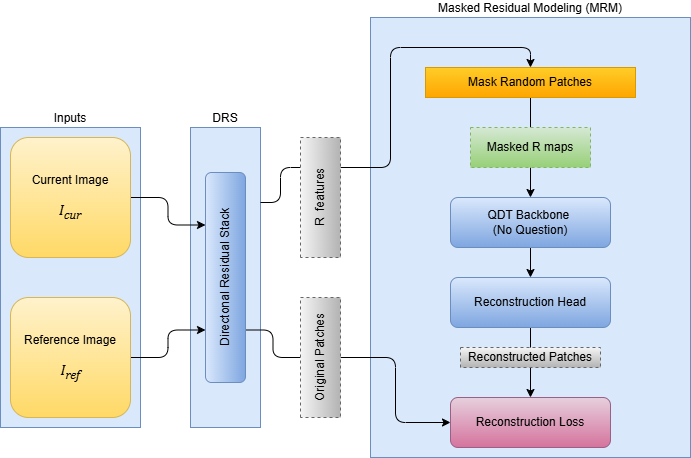
\includegraphics[width=0.9\textwidth]{figures/mrm.png}
	\caption{Masked Residual Modeling}
	\label{fig:mrm}
\end{figure}

\section{Multi-Stage Training Strategy}
The model is optimized using a comprehensive four-stage training regimen to ensure model robustness, prevent shortcut learning, and explicitly ground the vision-language alignment, 

To enforce contextual coherence in the visual representation, 50 percent of the residual tokens are randomly masked in the first stage. A lightweight reconstructor is trained to predict the masked tokens from the visible context using a Mean Squared Error (MSE) objective ($\mathcal{L}_{mrm}$). 

In second stage, a multi-label classification head is attached to predict 14 standard thoracic diseases from both the reference and current features using a Binary Cross-Entropy loss ($\mathcal{L}_{cls}$) to explicitly ground the visual features in known pathology 

To mitigate spurious correlations and dataset biases and hallucinations, the model applies a combination of hierarchical Kullback-Leibler (KL) divergence and Noise Contrastive Estimation (NCE) in third stage. By contrasting true longitudinal pairs against synthetically perturbed counterfactual pairs, the model disentangles true temporal evolution from visual noise ($\mathcal{L}_{cf}$). 

In the last stage, the entire architecture is fine-tuned for the generation task using a standard language cross-entropy loss ($\mathcal{L}_{lang}$) alongside an L1 sparsity regularization penalty on the gating weights ($\mathcal{L}_{gate}$) to force the gate to actively suppress non-essential information. The total loss of the complete training objective is weighted sum of these components.
\begin{equation}
	\mathcal{L}_{total} = \lambda_{lang}\mathcal{L}_{lang} + \lambda_{gate}\mathcal{L}_{gate} + \lambda_{mrm}\mathcal{L}_{mrm} + \lambda_{cls}\mathcal{L}_{cls} + \lambda_{cf}\mathcal{L}_{cf}
\end{equation}

\section{Implementation Details}
To ensure full reproducibility, ALIGN-VQA was developed using \cite{pytorch}. The model features a highly efficient parameter footprint of approximately 182.5M parameters. The QDT module retains a maximum of 64 tokens during early training, which is dynamically pruned to $K=16$ during fine-tuning. The maximum generated answer length is constrained to 128 tokens. Optimization is performed using the AdamW optimizer with a batch size of 128 and an initial learning rate of $5 \times 10^{-5}$, governed by a cosine annealing learning rate scheduler. The training schedule consists of 1 epoch of MRM, 3 warm-up epochs, and 20 epochs of end-to-end VQA fine-tuning. The empirically derived loss weights are set to $\lambda_{lang}=1.0$, $\lambda_{mrm}=0.1$, $\lambda_{cf}=0.1$, and $\lambda_{cls}=0.5$. Vocabulary mismatch issues during inference are handled dynamically by matching the initialized target vocabulary dimension to the exact embedding size preserved in the saved model checkpoints.
